\documentclass[fr]{../../../../../../eplexam}
\usepackage[american]{circuitikz}
\usepackage{siunitx}
\usepackage{etoolbox}
\usepackage{tikz}

\newcommand{\midarrow}{\tikz \draw[-stealth'] (0,0) -- +(.1,0);}

\usetikzlibrary{arrows}


\makeatletter

\pgfcircdeclarebipole{}
{\ctikzvalof{bipoles/tline/height}}{tline}
{\ctikzvalof{bipoles/tline/height}}
{\ctikzvalof{bipoles/tline/width}}
{   
	%% First find distance from startpoint to endpoint
	\pgfpointdiff{\pgfpointanchor{\ctikzvalof{bipole/name}start}{center}}
	{\pgfpointanchor{\ctikzvalof{bipole/name}end}{center}}
	\pgfmathparse{veclen(\the\pgf@x,\the\pgf@y)}
	%% The coordinate system has been changed so that the origin is at the midpoint and
	%% the line is along the x axis. So shift back by half the length of the line, and 
	%% make the cylinder of width roughly the length of the line, with a 40pt setback
	%% on each side.
	\pgftransformxshift{\pgfmathresult/2-30pt}
	\pgf@circ@res@left=\dimexpr-\pgfmathresult pt+40pt\relax
	%% Here is the original function, copied directly from the source of circuittikz, 
	%% down to next %%
	\pgf@circ@res@step=.2\pgf@circ@res@right % half x axis
	\pgfsetlinewidth{\pgfkeysvalueof{/tikz/circuitikz/bipoles/thickness}\pgfstartlinewidth}
	\pgfpathellipse{\pgfpoint{\pgf@circ@res@right-\pgf@circ@res@step}{0}}
	{\pgfpoint{\pgf@circ@res@step}{0}}
	{\pgfpoint{0}{-\pgf@circ@res@up}}
	\pgfpathmoveto{\pgfpoint{\pgf@circ@res@right-\pgf@circ@res@step}{\pgf@circ@res@up}}
	\pgfpathlineto{\pgfpoint{\pgf@circ@res@left+\pgf@circ@res@step}{\pgf@circ@res@up}}
	\pgfpatharc{-90}{90}{-\pgf@circ@res@step and -\pgf@circ@res@up}
	\pgfpathlineto{\pgfpoint{\pgf@circ@res@right-\pgf@circ@res@step}{\pgf@circ@res@down}}
	%% I have to fill the figure to block out the original line
	\pgfsetfillcolor{white}
	\pgfusepath{draw,fill}
	%% Redraw part of the line that gets blocked by the cylinder by mistake
	\pgfpathmoveto{\pgfpoint{\pgf@circ@res@right-2*\pgf@circ@res@step}{0pt}}
	\pgfpathlineto{\pgfpoint{\pgf@circ@res@right}{0pt}}
	\pgfusepath{draw}
}

\hypertitle{Electromagnétisme}{5}{ELEC}{1350}{2017}{Août}{All}
{Martin Braquet}
{Christophe Craeye et Danielle Janvier}

\section{Lignes de transmission en transitoire}

\begin{center}
	\begin{circuitikz}
		
		\draw[thick]
		(-1,0) -- (5,0)
		(-1,2) to[V_=5V,-*] (-1,0)
		(-1,2) to[R=\SI{50}{\Omega}] (1,2)
		(-1,0) node[ground] {}
		(1,2) -- (2,3)
		(2,2) -- (4,2) 
		to [TL] (8,2) -- (10,2)
		to [TL] (14,2)
		to[R=\SI{25}{\Omega}] (14,0)
		(4,0) to [TL] (8,0) -- (10,0)
		to [TL] (14,0)
		(9,0) to[R,a=\SI{50}{\Omega},*-*] (9,2)
		(2.5,2) to[short,*-] (3.75,-0.5)
		to [TL] (5.5,-4)
		(2.5,0) to[short,*-] (3,-1)
		to [TL] (4.75,-4.5)
		-- (5.5,-4)
		(3,2) node[anchor=south] {$V_o$}
		(6,1) node {$Z_0=\SI{50}{\Omega}$}
		(12,1) node {$Z_0=\SI{50}{\Omega}$}
		(6,-2) node {$Z_0=\SI{50}{\Omega}$}
		(3,-3) node {\SI{15}{cm}}
		(6,-0.5) node {\SI{10}{cm}}
		(12,-0.5) node {\SI{25}{cm}}
		;
		
	\end{circuitikz}
\end{center}

On considère que la permittivité relative des lignes vaut $\epsilon_r=4$.

\begin{enumerate}
	\item Calculer $V_o$ après \SI{3}{ns}.
	\item Que vaut la tension du générateur en sortie en régime ?
	\item Après avoir coupé le générateur en régime, que vaut $V_o$ durant \SI{3}{ns}?
\end{enumerate}

\begin{solution}
	
\begin{enumerate}
	\item On numérote les lignes de 1 à 3 par ordre croissant de leur longueur. On a deux branches en parallèle, la tension $V_o$ est donc la somme de la tension générée par la source et des ondes réfléchies des deux lignes. On peut établir deux diagrammes, un par branche:
	
	\begin{center}
	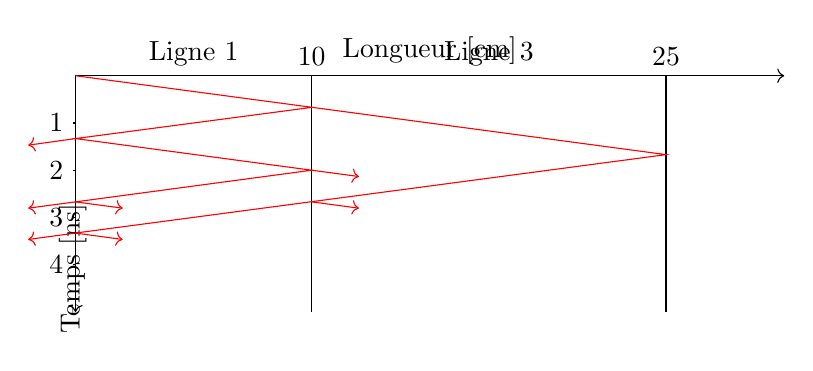
\begin{tikzpicture}[scale=0.3]
		\draw[->] (0,0) -- coordinate (x axis mid) (30,0);
		\draw[->] (0,0) -- coordinate (y axis mid)(0,-10);
		\foreach \x in {10,25}
		\draw (\x,-10) -- (\x,0)
		node[anchor=south] {\x};
		\foreach \y in {1,2,3,4}
		\draw (0,-\y*2 ) -- (-3pt,-\y*2) node[anchor=east] {\y};
		\node[above=0.5] at (x axis mid) {Longueur [cm]};
		\node[above] at (5,0) {Ligne 1};
		\node[above] at (17.5,0) {Ligne 3};
		\node[left=1,rotate=90] at (y axis mid) {Temps [ns]};
		\draw[color=red] 
		(0,0) -- (25,-1.67*2) -- (0,-3.33*2)
		(10,-0.67*2) -- (0,-1.33*2) -- (10,-2*2) -- (0,-2.67*2)
		;
		\draw[->,color=red] (10,-2*2) -- (12,-2.1333*2);
		\draw[->,color=red] (0,-1.33*2) -- (-2,-1.47*2);
		\draw[->,color=red] (10,-2.67*2) -- (12,-2.8033*2);
		\draw[->,color=red] (0,-2.67*2) -- (2,-2.8033*2);
		\draw[->,color=red] (0,-2.67*2) -- (-2,-2.8033*2);
		\draw[->,color=red] (0,-3.33*2) -- (2,-3.466*2);
		\draw[->,color=red] (0,-3.33*2) -- (-2,-3.466*2);
	\end{tikzpicture}
	\end{center}

	\begin{center}
	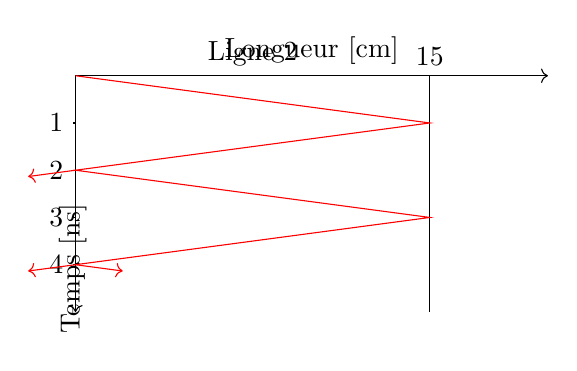
\begin{tikzpicture}[scale=0.3]
		\draw[->] (0,0) -- coordinate (x axis mid) (20,0);
		\draw[->] (0,0) -- coordinate (y axis mid)(0,-10);
		\node[above] at (7.5,0) {Ligne 2};
		\foreach \x in {15}
		\draw (\x,-10) -- (\x,0)
		node[anchor=south] {\x};
		\foreach \y in {1,2,3,4}
		\draw (0,-\y*2 ) -- (-3pt,-\y*2) node[anchor=east] {\y};
		\node[above=0.5] at (x axis mid) {Longueur [cm]};
		\node[left=1,rotate=90] at (y axis mid) {Temps [ns]};
		\draw[color=red] 
		(0,0) -- (15,-1*2) -- (0,-2*2) -- (15,-3*2) -- (0,-4*2)
		;
		\draw[->,color=red] (0,-4*2) -- (2,-4.1333*2);
		\draw[->,color=red] (0,-2*2) -- (-2,-2.1333*2);
		\draw[->,color=red] (0,-4*2) -- (-2,-4.1333*2);
	\end{tikzpicture}
	\end{center}
	
	En considérant que la permittivité relative des lignes vaut $\epsilon_r=4$, les temps pour traverser les lignes valent $t_{10}=0.1\sqrt{\epsilon_r}/c=\SI{0.67}{ns},t_{15}=0.15\sqrt{\epsilon_r}/c=\SI{1}{ns}$ et $t_{25}=0.25\sqrt{\epsilon_r}/c=\SI{1.67}{ns}$.
	
	La tension $V_o$ initiale vaut $$5\frac{(50//50)}{(50//50)+50}=5/3$$ car les impédances des lignes 1 et 2 sont en parallèle.
	On calcule les coefficient de réflexion, par exemple le premier correspond à la ligne 1 vers le générateur:
	\[
		\Gamma_{1\rightarrow s}=\frac{(50//50)-50}{(50//50)+50}=-1/3
	\]
	\[
	\Gamma_{1\rightarrow 3}=\frac{(50//50)-50}{(50//50)+50}=-1/3
	\]
	\[
	\Gamma_{3\rightarrow L}=\frac{25-50}{25+50}=-1/3
	\]
	\[
	\Gamma_{3\rightarrow 1}=\frac{(50//50)-50}{(50//50)+50}=-1/3
	\]
	\[
	\Gamma_{2\rightarrow L}=\frac{0-50}{0+50}=-1
	\]
	\[
	\Gamma_{2\rightarrow s}=\frac{(50//50)-50}{(50//50)+50}=-1/3
	\]
	
	L'onde transmise au générateur à \SI{1.33}{ns} venant de la ligne 1 vaut $$\frac{5}{3}\cdot\frac{-1}{3}\cdot\left(1+\frac{-1}{3}\right)=\SI{-0.37}{V}$$
	L'onde transmise au générateur à \SI{2.67}{ns} venant de la ligne 1 vaut $$\frac{5}{3}\cdot\frac{-1}{3}\cdot\frac{-1}{3}\cdot\frac{-1}{3}\cdot\left(1+\frac{-1}{3}\right)=\SI{-0.04}{V}$$
	L'onde transmise au générateur à \SI{2}{ns} venant de la ligne 2 vaut $$\frac{5}{3}\cdot(-1)\cdot\left(1+\frac{-1}{3}\right)=\SI{-1.11}{V}$$
	La tension $V_o$ après \SI{3}{ns} vaut donc $$\frac{5}{3}-0.37-0.04-1.11=\SI{0.146}{V}$$
	
	
	\item On calcule la somme de toutes les ondes transmises au générateur. Comme il n'est pas évident de trouver une série géométrique qui convienne pour 2 lignes de transmission en série, on utilise le raisonnement suivant.
	
	\begin{center}
		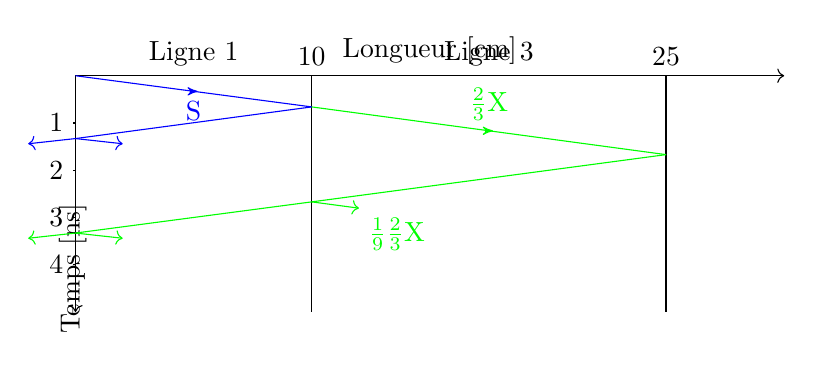
\begin{tikzpicture}[scale=0.3]
		\draw[->] (0,0) -- coordinate (x axis mid) (30,0);
		\draw[->] (0,0) -- coordinate (y axis mid)(0,-10);
		\foreach \x in {10,25}
		\draw (\x,-10) -- (\x,0)
		node[anchor=south] {\x};
		\foreach \y in {1,2,3,4}
		\draw (0,-\y*2 ) -- (-3pt,-\y*2) node[anchor=east] {\y};
		\node[above=0.5] at (x axis mid) {Longueur [cm]};
		\node[above] at (5,0) {Ligne 1};
		\node[above] at (17.5,0) {Ligne 3};
		\node[left=1,rotate=90] at (y axis mid) {Temps [ns]};
		\draw[color=blue] (0,0) -- node {\midarrow} coordinate (c1) (10,-0.66*2);
		\draw[color=blue] (0,-1.33*2) -- (10,-0.66*2);
		\draw[->,color=blue] (0,-1.33*2) -- (2,-1.44*2);
		\draw[->,color=blue] (0,-1.33*2) -- (-2,-1.44*2);
		\draw[color=blue] node[below] at (c1){S};
		\draw[color=green] (10,-0.66*2) -- node {\midarrow} coordinate (c1) (25,-1.67*2);
		\draw[color=green] (25,-1.67*2) -- (10,-2.67*2);
		\draw[color=green] (0,-3.33*2) -- (10,-2.67*2);
		\draw[->,color=green] (0,-3.33*2) -- (-2,-3.44*2);
		\draw[->,color=green] (0,-3.33*2) -- (2,-3.44*2);
		\draw[color=green] node[above] at (c1){$\frac{2}{3}$X};
		\draw[->,color=green] (10,-2.67*2) -- (12,-2.8033*2) node[anchor=north west] (){$\frac{1}{9}\frac{2}{3}$X};
		\end{tikzpicture}
	\end{center}

	Soit $S$, la somme de toutes les ondes transmises à la source pour une tension initiale de \SI{1}{V} à l'entrée de la ligne 1. Et soit $X$, la somme de toutes les ondes transmises à la source pour une tension initiale de \SI{1}{V} à l'entrée de la ligne 3. On a donc les relations $$ S=\frac{2}{3}X+\frac{-1}{3}\cdot\left(1+\frac{-1}{3}\right)+\frac{-1}{3}\cdot\frac{-1}{3}S $$
	et
	$$ X= \frac{-1}{3}\cdot\frac{-1}{3}X+\frac{-1}{3}\cdot\left(1+\frac{-1}{3}\right)\cdot\left(1+\frac{-1}{3}\right)+\frac{-1}{3}\cdot\left(1+\frac{-1}{3}\right)\cdot\frac{-1}{3}S$$
	On trouve ainsi que $S=-2/5$. Puisqu'il y a une tension de \SI{5/3}{V} à l'entrée. La somme des ondes transmises venant de la ligne 1 vaut $ \frac{-2}{5}\frac{5}{3}=\SI{-0.67}{V}$.
	
	Pour les ondes de la lignes 2, elles valent
	$$ \frac{5}{3}\left( (-1)\cdot\frac{2}{3}+(-1)\cdot\frac{-1}{3}\cdot(-1)\cdot\frac{2}{3}+(-1)\cdot\frac{-1}{3}\cdot(-1)\cdot\frac{-1}{3}\cdot(-1)\cdot\frac{2}{3}+\ldots \right)$$ $$= \frac{5}{3} \sum_{i=0}^{\infty}(-1)\left(\frac{1}{3}\right)^i\frac{2}{3}=\frac{5}{3}(-1)\frac{1}{1-\frac{1}{3}}\frac{2}{3}=-\frac{5}{3}$$
	Ce résultat est logique puisque la tension d'entrée en régime d'une ligne dont l'impédance de charge est nulle vaut 0.
	
	La tension $V_o$ de régime vaut donc $$\frac{5}{3}-\frac{5}{3}-0.67=\SI{-0.67}{V}$$
	
	\item En coupant le générateur, on supprime instantanément \SI{5/3}{V} à $V_o$, donc $V_o=\SI{-2.33}{V}$. L'onde parcourt le même trajet que dans la sous-question 1, il suffit juste de remplacer \SI{5/3}{V} par \SI{-2.33}{V}.
	
	L'onde transmise au générateur à \SI{1.33}{ns} (après la fermeture de la source) venant de la ligne 1 vaut $$-2.33\cdot\frac{-1}{3}\cdot\left(1+\frac{-1}{3}\right)=\SI{0.52}{V}$$
	L'onde transmise au générateur à \SI{2.67}{ns} (après la fermeture de la source) venant de la ligne 1 vaut $$-2.33\cdot\frac{-1}{3}\cdot\frac{-1}{3}\cdot\frac{-1}{3}\cdot\left(1+\frac{-1}{3}\right)=\SI{0.06}{V}$$
	L'onde transmise au générateur à \SI{2}{ns} (après la fermeture de la source) venant de la ligne 2 vaut $$-2.33\cdot(-1)\cdot\left(1+\frac{-1}{3}\right)=\SI{1.55}{V}$$
	La tension $V_o$ après \SI{3}{ns} (après la fermeture de la source) vaut donc $$-2.33+0.52+0.06+1.55=\SI{-0.2}{V}$$
\end{enumerate}
	
\end{solution}


\end{document}
